\documentclass[conference]{IEEEtran}
\IEEEoverridecommandlockouts
% The preceding line is only needed to identify funding in the first footnote. If that is unneeded, please comment it out.
%Template version as of 6/27/2024
\usepackage[T1]{fontenc}
\usepackage{tabularx,booktabs}
\usepackage{cite}
\usepackage{amsthm}
\newtheorem{definition}{Definition}
%\usepackage{amsmath,amssymb,amsfonts}
\usepackage{amsmath}

\usepackage{algorithm}
\usepackage{algorithmicx}
\usepackage[noend]{algpseudocode} % very import in IEEEtran
%\usepackage{algorithmic}
\usepackage{graphicx}
\usepackage{textcomp}
\usepackage{subfigure}
\usepackage[numbers, sort&compress]{natbib}
%\usepackage{natbib}
\usepackage{xcolor}
\usepackage{doi}
\usepackage{float}
\usepackage{lineno}
\usepackage{tikz}
\usepackage{tikz-qtree}
\usetikzlibrary{shapes, arrows, positioning, calc, shadows}
\usepackage{enumitem}
%\usepackage{subcaption} 

\usepackage{framed}
\usepackage{listings}
\usepackage{pgfplots}     % 核心绘图库
\pgfplotsset{compat=newest} % 版本兼容
\usepackage{filecontents} % 内嵌数据文件
\lstset{
    language=Verilog,
    %basicstyle=\ttfamily\scriptsize,
    basicstyle=\ttfamily\tiny,
    keywordstyle=\color{blue},
    commentstyle=\color{green!50!black}\tiny,
    stringstyle=\color{red},
    backgroundcolor=\color{green!10},
    showstringspaces=false,
    numbers=left,
    numberstyle=\tiny\color{gray},
    frame=single,
    breaklines=true,
    tabsize=4,
    columns=flexible, % 灵活列宽
    breaklines=false, % 不自动换行
    aboveskip=0pt, % 减少上方间距
    belowskip=0pt, % 减少下方间距
    captionpos=b
}

% 定义流程图样式
\tikzset{
    startstop/.style={
        rectangle, rounded corners=1mm, minimum width=2cm, minimum height=0.5cm, 
        align=center, draw=black, fill=red!20, drop shadow, 
        font=\sffamily\bfseries
    },
    process/.style={
        rectangle, minimum width=2cm, minimum height=0.5cm, 
        align=center, draw=black, fill=blue!20, drop shadow,
        font=\sffamily
    },
    decision/.style={
        diamond, aspect=1.5, minimum width=2cm, minimum height=1cm, 
        align=center, draw=black, fill=green!20, drop shadow,
        font=\sffamily
    },
    io/.style={
        trapezium, trapezium left angle=70, trapezium right angle=110, 
        minimum width=2cm, minimum height=0.5cm, align=center, 
        draw=black, fill=yellow!20, drop shadow,
        font=\sffamily
    },
    database/.style={
        cylinder, shape border rotate=90, aspect=0.3, 
        minimum width=1.5cm, minimum height=1.5cm, 
        draw=black, fill=orange!20, drop shadow,
        font=\sffamily
    },
    connector/.style={
        ellipse, minimum width=1cm, minimum height=1cm, 
        align=center, draw=black, fill=purple!20, drop shadow,
        font=\sffamily\small
    },
    arrow/.style={
        thick, -{stealth[scale=1.2]}, line width=1pt
    },
    dashedarrow/.style={
        arrow, dashed, green!50!black
    },
    note/.style={
        rectangle, rounded corners=2mm, draw=gray!50, fill=yellow!10, 
        inner sep=5pt, align=left, font=\small\sffamily,
        text width=3.5cm
    },
    straightline/.style = {line width = 1pt,-},
    point/.style={coordinate}
}

\def\BibTeX{{\rm B\kern-.05em{\sc i\kern-.025em b}\kern-.08em
    T\kern-.1667em\lower.7ex\hbox{E}\kern-.125emX}}
\begin{document}

\title{Dataflow-Based Path Pruning in Symbolic Execution for Hardware Verification%*\\
%{\footnotesize \textsuperscript{*}Note: Sub-titles are not captured for https://ieeexplore.ieee.org  and
%should not be used}
%\thanks{Identify applicable funding agency here. If none, delete this.}
}

%\author{\IEEEauthorblockN{1\textsuperscript{st} Jiahui Liang}
%\IEEEauthorblockA{\textit{Institute of Software} \\
%\textit{Chinese Academy of Sciences}\\
%Beijing, China \\
%jiahui@iscas.ac.cn}
%\and
%\IEEEauthorblockN{2\textsuperscript{nd} Qiusong Yang}
%\IEEEauthorblockA{\textit{Institute of Software} \\
%\textit{Chinese Academy of Sciences}\\
%Beijing, China \\
%qiusong@iscas.ac.cn}
%\and
%\IEEEauthorblockN{3\textsuperscript{rd} Yiwei Ci}
%\IEEEauthorblockA{\textit{Institute of Software} \\
%\textit{Chinese Academy of Sciences}\\
%Beijing, China \\
%yiwei@iscas.ac.cn}
%}
\IEEEspecialpapernotice{\vspace{-2em}}
\author{
Jiahui Liang$^{1,2}$, Qiusong Yang$^{1,2*}$, Yiwei Ci$^{1,2}$    \\
$^{1}$Institute of Software, Chinese Academy of Sciences, Beijing, China \\
$^{2}$University of Chinese Academy of Sciences, Beijing, China \\
*Corresponding Author: qiusong@iscas.ac.cn
}
%\IEEEaftertitletext{\vspace{-2em}}
\IEEEaftertitletext{}

%\vspace{5pt}
\maketitle

\begin{abstract}
Ensuring the security of modern SoCs is increasingly critical, yet verifying security behaviors at the hardware level remains highly challenging due to complex RTL interactions and limited coverage of traditional methods. Symbolic execution is a powerful verification technique that systematically explores all feasible paths, yet it has faced the critical challenge of path explosion since its emergence. Recent work has begun to focus on performing verification directly on RTL source code, explicitly exploiting RTL-specific characteristics, such as exploit independent modules in RTL designs to reduce path exploration by avoiding re-execution of identical modules. However, these techniques cannot eliminate redundant path explorations within individual modules. To address this limitation, we propose a dataflow-based symbolic execution technique for efficient path exploration. Our approach targets on combinational logic circuits and introduces a novel pruning strategy based on forward dataflow analysis to  to avoid redundant path exploration. We evaluate our approach on two open-source RISC-V cores(PICORV32 and DarkRISCV) and a SoC design. Experimental results demonstrate that our technique reduces path exploration by approximately 10\% to 34\%.
\end{abstract}

\begin{IEEEkeywords}
Symbolic Execution, Hardware Verification, SoC Security.
\end{IEEEkeywords}
\vspace{-8pt}
\section{Introduction}
%The verification is crucial in the development of hardware. The mainstream verification methods are simulation-based verification and formal verification\cite{introduction_1}. Simulation-based verification normally utilizes random or well-designed test cases to cover the states of a DUV(Design under Verification). Formal verification normally explore all the possible states of DUV to prove whether it satisfies specific properties.  
In modern IoT, automotive, and embedded platforms, System-on-Chip (SoC) devices constitute the root of trust responsible for safeguarding security-critical assets such as cryptographic keys, configuration registers, privilege states, and secure-world boundaries. Since these assets are ultimately controlled by RTL-level hardware logic, vulnerabilities originating at the RTL layer can compromise the entire security stack, leading to information leakage, privilege escalation, or persistent exploitation\cite{chen_challenges_2017}. Ensuring the correctness of RTL hardware security mechanisms has therefore become a central objective in contemporary SoC development.

However, RTL designs present inherent challenges for security verification. Security semantics frequently rely on subtle multi-cycle dependencies, implicit information flows, cross-domain interactions (e.g., power/clock/reset), and dynamically reconfigurable logic \cite{farahmandi_system--chip_2020}. Such behaviors are difficult for simulation-driven verification to capture, as simulation provides limited coverage of deep, security-relevant corner cases. Symbolic execution, as a formal technique capable of systematically exploring RTL control and data paths, offers appealing benefits in detecting unauthorized information flow, invalid state transitions, and subtle violations that evade conventional testing\cite{co-verif}\cite{soc-verif}.
%Symbolic execution replaces concrete input values with symbols, each of which representing the set of possible values of an input parameter. A symbolic execution engine drives the process using the semantics of the programming language, extended to handle symbols. During execution, symbols are used instead of literal values. When encountering a branch point (e.g., an if statement), both paths are explored separately. The result of symbolically executing a design for one clock cycle is a tree of paths, each associated with a unique path condition describing the branch decisions required to follow that path. Symbolic execution is frequently used to detect assertion violations. If any path violates an assertion, its path condition precisely describes the inputs that would drive concrete execution down that same violating path. Concrete values satisfying this condition constitute a counter-example to the assertion\cite{soc-verif}.

%Symbolic execution has become a widely used technique in hardware verification. Notably recent advances include the use of path-based symbolic execution for hardware/software co-verification, which partitions firmware and hardware logic to generate concise formulas and significantly accelerates verification compared to traditional bounded model checking approaches \cite{co-verif}. The process of symbolic execution is driven by symbolic execution engines, such as KLEE\cite{klee}, which have been integrated with RTL designs and instruction set simulators to uncover functional mismatches and bugs in RISC-V processors, demonstrating the scalability and effectiveness of symbolic execution in embedded hardware\cite{concolic_1}. Symbolic execution has been applied to accelerate SoC security verification by converting hardware designs to C++ and selectively symbolizing critical inputs, enabling efficient vulnerability detection\cite{soc-verif}. 


 Despite its advantages, symbolic execution suffers from the same fundamental scalability limitations that constrain other formal methods.Two factors lead to the path explosion problem. One is the inherent high complexity of DUV(Design Under Verification), which is inevitable. The other factor is that these approaches verify the a software model of hardware designs, using a symbolic execution engine for software analysis, such as KLEE, to explore the possible paths. The symbolic execution engine for software sequentially updates the execution paths and query the SMT solver frequently and ignores that the huge amount of independent always blocks in hardware, which can explore the paths in parallel. Hence, path explosion problem gets even worse because a huge amount of paths are re-explored, and invokes  the SMT solver in vain. The latest symbolic execution engine, Sylvia \cite{Ryan2023Sylvia}, leverages the independence of always blocks to reduce the re-explorations of the same paths. Sylvia explores the paths of each always block separately and combines them to generate the final paths. However, Sylvia only solves the re-exploration problem of path by leveraging the explore the independent always blocks in parallel. Given n independent always blocks, the amount of total path is $\prod_{i=1}^{n} p_i $ where $p_i$ represents the amount of path of a single always block $i$. We use $r_i$ to represent the portion of the remnant paths after path pruning in always block $i$, the percentage of the remnant path equals $\prod_{i=1}^{n} r_i$($r_i \leq  1$), there is a huge space to reduce the paths to explore.

%In our approach, we target the always blocks describing the combinational logic, in which the statements are sequentially executed. With the analysis of the final states of the outputs in the motivating example, we observe that the combination of independent branches produces different path leading to the same state. To identify independent branches in the same always block, we analyze the dependence relations between different branches in the hardware design.  Then we leverages the dependence analysis to prune the redundant paths leading to the same states.
In our approach, we focus on always blocks that describe combinational logic, where the statements are executed sequentially. From the motivating example, we observe that different combinations of branch outcomes can still drive the design to the same state at the outputs. To capture this effect within a single always block, we analyze how branch conditions propagate through assignments and which statements they can influence. The resulting dataflow information is then used during symbolic execution to recognize path segments whose exploration would not produce any new states, so that these redundant paths can be safely pruned.

To summarize, the contributions of this paper are:
%\begin{itemize}[itemsep=2pt, topsep=0pt, parsep=1pt]
\begin{itemize}[itemsep=1pt, topsep=1pt, parsep=0pt,leftmargin=*]

%\begin{itemize}[topsep=2pt]
\item We observe and illustrate that in a hardware design, the combination of some branches may produce different path leading to the same state. We can do the dataflow analysis to identify and prune these redundant paths.
\item We propose a pruning strategy to reduce the number of paths to be explored by dataflow analysis in each always blocks in the hardware design.
\item We implement our approach on the top of a symbolic execution engine, Sylvia, and evaluate its performance on two open-sourced RISC-V cores(PICORV32 and DarkRISCV), and an SoC design from HACK@DAC'18. The experimental results show that our approach can significantly reduce from about 10\%  to nearly 34\% of paths explored on these three RTL designs by Sylvia. %while maintaining the same bug detected ability.
\end{itemize}
The rest of the paper is organized as follows: In Section \ref{sec:motivation}, we provide an example to show the basic flow of hardware symbolic execution and the redundant paths introduced by combinational logic. In Section \ref{sec:strategy}, we present our method to reduce the redundant paths in combinational logic. In section \ref{sec:evaluation}, we evaluate our method and show its effect. In section \ref{sec:related_work}, we summarize related works. We conclude our work in section \ref{sec:conclusion}.

\section{Preliminaries and Motivation}
\label{sec:motivation}
%In this section, we first introduce the background of symbolic execution and knowledge of the Verilog assignments. 

In this section, we briefly introduce the symbolic execution on hardware, and use an example to illustrate the procedure during execution.
\subsection{Symbolic Execution on Hardware}
Symbolic execution on hardware is conducted by a symbolic execution engine, which maintains and updates the symbolic states $s$, where:
\begin{itemize}[topsep=1pt]
    \item $stmt$ is the next statement to evaluate. In an symbolic execution engine for hardware, $stmt$ can be an non-blocking assignment, blocking assignment, or a branch. 
    \item $\sigma$ is a $symbolic \ store$ that maps variables to concrete values or symbolic values $\alpha_{i}$.
    \item $\pi$ is called $path \  constraints$, which is a formula expressing a set of assumptions on symbols $\alpha_{i}$. $path constraint$ is determined by the choices on each branch.
\end{itemize}

Symbolic execution engine for hardware analyzes the hardware designs directly on RTL(Register Transfer Level), rather than a software model translated by EDA tools, through which the normal symbolic execution engines analyze the hardware designs. The field of $stmt$ differs the state during a software symbolic execution, in which there is only one type of assignment. 

The assignments in RTL can be classified into blocking assignment and non-blocking assignment: Blocking assignments are used to model combinational logic, denoted by the operator "=", and executed sequentially in the order they are stated. The blocking assignments update the left-hand variable immediately. 
Non-blocking assignments are used to model sequential logic, denoted by the operator "<=", and are executed in parallel, not following the order of statements. In this work we only focus on blocking assignments during one cycle, hence we do not make a further discussion on non-blocking assignments.% Non-blocking assignments do not update the left-hand variable at the current cycle, but at the start of next cycle.

%With an assumption that current execution is at cycle ${i}$, the hardware symbolic execution engine updates the state $s$ according to the type of $stmt$:
The hardware symbolic execution engine updates the symbolic state $s$ according to the type of $stmt$:

\begin{itemize}[itemsep=2pt, topsep=0pt, parsep=1pt]
    \item The evaluation of variable $x$ with a blocking assignment $x := e$ updates the symbolic store $\sigma$ immediately by assigning $x$ with a expression $e$, where $e$ can be calculated through the context of the current symbolic state. 
    \item The evaluation of a conditional branch $if_e$ affects the path constraints $\pi$. The symbolic execution is forked from both the $taken$ and $not\ taken$ of the $if_e$, forking two new execution states with new path constraint $\pi_{true} = \pi \land e_s$ and $\pi_{false}=\pi \land \lnot e_s$ respectively. 
\end{itemize}

The symbolic execution of a hardware explores the hardware design only for one clock cycle, hence the symbolic execution engine on hardware behaves as a loop, updating state $s$ cycle by cycle. At beginning of the current cycle,  $e_s$ is the evaluation of $e$ with the context related with state $s$, which gets initialized by the values of registers, and non-blocking assignments from the previous cycle.
Same to the software symbolic execution engine, path constraint $\pi$ is initialized to $True$, and symbolic store $\sigma$ associates all the variables to 0 at cycle 0. 

%\subsection{dataflow Analysis}
%dataflow analysis is the process of collecting information about the way the variables are defined and used in the program. It attempts to obtain particular information at each point in a procedure. 
\vspace{-3mm}
\subsection{Motivating Example}
In this section, we present a simple example of combinational logic to illustrate the basic process of hardware symbolic execution engine e.g. Sylvia and present the redundant paths during the process in Figure \ref{fig:path-all}. The Verilog RTL is given in Figure \ref{fig:verilog-fig}. The hardware design consists of two always blocks, both of them represent combinational logic. 

As mentioned before, the previous work leverages the independence between two always blocks to reduce the paths to explore. As shown in Figure \ref{fig:path-all}, it explores the first always block and the second always block separately. Figure \ref{fig:paths-a} and Figure \ref{fig:paths-b} present the execution trees of the first and the second always block respectively. While the symbolic execution engine for software explore these two always block sequentially, forking new states from conditional branch at line 24 to explore the second always block. Through this approach, sub-trees rooted from nodes labeled with 24 are executed 8 times, which costs extra resources and time. But Sylvia only explores each tree once, only combines two sub-paths from two different trees with a SMT query to check whether the path constraints are feasible.


\begin{figure*}[h!]
\centering
\resizebox{0.9\textwidth}{!}{
    \subfigure[Execution Tree of the First Always Block]{
        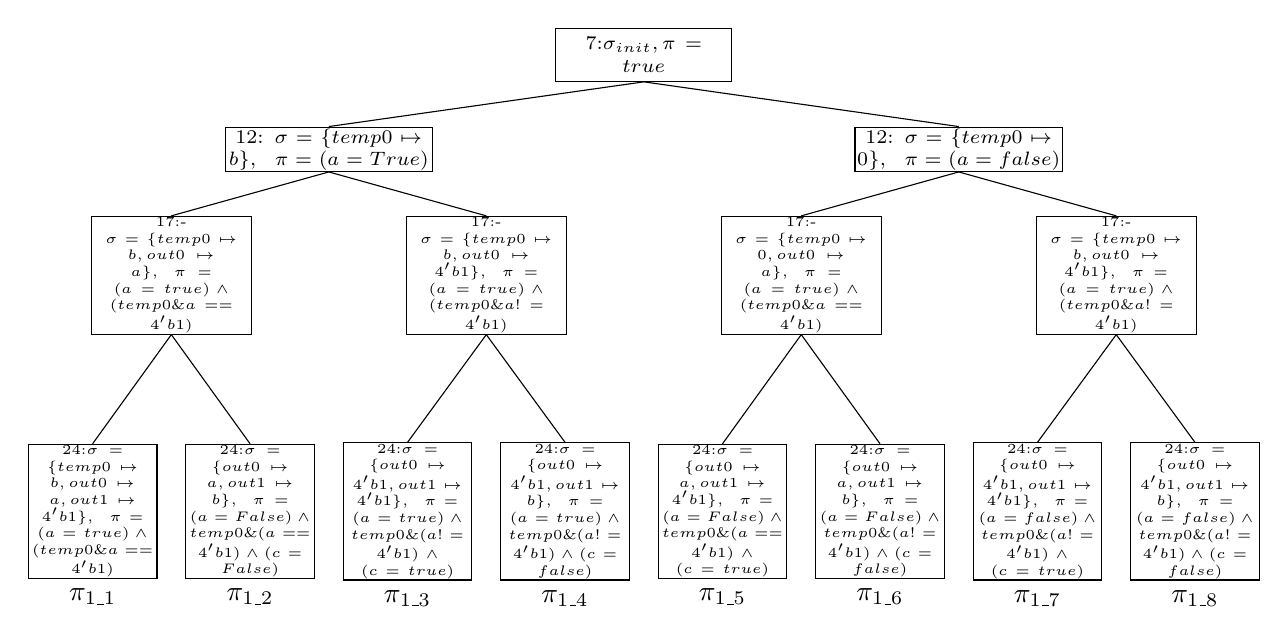
\begin{tikzpicture}[
            %level distance=20mm,
            level 1/.style = {sibling distance=80mm, level distance=12mm},
            level 2/.style = {sibling distance=40mm, level distance=16mm},
            level 3/.style = { level distance=30mm},
            every node/.style = {
                draw, rectangle,
                rounded corners=3pt,
                %minimum size=15mm,       % Increased size
                minimum width=15mm,
                text width=10mm,
                minimum height=5mm,
                inner sep=0.5pt,
                align=left
                %font=\small
            }
            leaf label/.style={
                font=\footnotesize,
                draw=none,
                minimum_size=1mm,
                below=2mm
            }
        ]
        \node [text width=20mm, align=center, draw, rectangle, font=\scriptsize]{7:$\sigma_{init}, \pi=true$}
            child {
                node [text width=26mm, align=center, draw, rectangle, font=\scriptsize, inner sep=0.5pt]{12:\- $\sigma=\{temp0 \mapsto b\},\ \  \pi=(a=True)$ }
                %edge from parent node[edge label, above left] {$choice A$}
                child { %node {17:$\pi_{1\_1}$}
                    node [text width=20mm, align=center, draw, rectangle, font=\tiny, inner sep=0.5pt]{17:\- $\sigma=\{temp0 \mapsto b, out0 \mapsto a\},\ \  \pi=(a=true) \land (temp0 \& a == 4'b1)$ }
                    [sibling distance=20mm]
                    child {
                        %node[label=below:$leaf$] {24}
                        %node [text width=15mm, align=center, draw, rectangle, font=\scriptsize, inner sep=0.5pt, label=below:$\pi_{1\_1}$]{24:$\sigma=\{temp0 \mapsto b, out0 \mapsto a, out1 \mapsto 4'b1\},\ \  \pi=(a=false) \land (temp0 \& a == 4'b1)$ }
                        node [text width=16mm, align=center, draw, rectangle, font=\tiny, inner sep=0.5pt, label=below:$\pi_{1\_1}$]{24:$\sigma=\{temp0 \mapsto b, out0 \mapsto a, out1 \mapsto 4'b1\},\ \  \pi=(a=true) \land (temp0 \& a == 4'b1)$ }
                        }
                    child {
                        %node [draw, rectangle, font=\tiny, label=below:$\pi_{1\_2}$]{24}
                        node [text width=16mm, align=center, draw, rectangle, font=\tiny, inner sep=0.5pt, label=below:$\pi_{1\_2}$]{24:$\sigma=\{out0 \mapsto a, out1 \mapsto b\},\ \  \pi=(a=False) \land temp0 \& (a == 4'b1) \land (c=False)$}
                    }
                }       
                child { 
                    %node[draw, circle, font=\tiny] {17}
                    node [text width=20mm, align=center, draw, rectangle, font=\tiny, inner sep=0.5pt]{17:\- $\sigma=\{temp0 \mapsto b, out0 \mapsto 4'b1\},\ \  \pi=(a=true) \land (temp0 \& a != 4'b1)$ }
                    [sibling distance=20mm]
                    child {
                        %node [draw, rectangle, font=\tiny, label=below:$\pi_{1\_3}$]{24}
                        node [text width=16mm, align=center, draw, rectangle, font=\tiny, inner sep=0.5pt, label=below:$\pi_{1\_3}$]{24:$\sigma=\{out0 \mapsto 4'b1, out1 \mapsto 4'b1\},\ \  \pi=(a=true) \land temp0 \& (a != 4'b1) \land (c=true)$}
                        }
                    child {
                    %node [draw, rectangle, font=\tiny, label=below:$\pi_{1\_4}$]{24}
                    node [text width=16mm, align=center, draw, rectangle, font=\tiny, inner sep=0.5pt, label=below:$\pi_{1\_4}$]{24:$\sigma=\{out0 \mapsto 4'b1, out1 \mapsto b\},\ \  \pi=(a=true) \land temp0 \& (a != 4'b1) \land (c=false)$}
                    }
                }
            }
            child {
                node [text width=26mm, align=center, draw, rectangle, font=\scriptsize, inner sep=0.5pt]{12:\- $\sigma=\{temp0\mapsto 0\},\ \  \pi=(a=false)$ }
                child { 
                    %node[draw, circle, font=\tiny] {17}
                    node [text width=20mm, align=center, draw, rectangle, font=\tiny, inner sep=0.5pt]{17:\- $\sigma=\{temp0 \mapsto 0, out0 \mapsto a\},\ \  \pi=(a=true) \land (temp0 \& a == 4'b1)$ }
                    [sibling distance=20mm]
                    child {
                        %node [draw, rectangle, font=\tiny, label=below:$\pi_{1\_5}$]{24}
                        node [text width=16mm, align=center, draw, rectangle, font=\tiny, inner sep=0.5pt, label=below:$\pi_{1\_5}$]{24:$\sigma=\{out0 \mapsto a, out1 \mapsto 4'b1\},\ \  \pi=(a=False) \land temp0 \& (a == 4'b1) \land (c=true)$}
                        }
                    child {
                        %node [draw, rectangle, font=\tiny, label=below:$\pi_{1\_6}$]{24}
                        node [text width=16mm, align=center, draw, rectangle, font=\tiny, inner sep=0.5pt, label=below:$\pi_{1\_6}$]{24:$\sigma=\{out0 \mapsto a, out1 \mapsto b\},\ \  \pi=(a=False) \land temp0 \& (a != 4'b1) \land (c=false)$}
                        }
                }
                child { 
                    %node [draw, circle, font=\tiny] {17}
                    node [text width=20mm, align=center, draw, rectangle, font=\tiny, inner sep=0.5pt]{17:\- $\sigma=\{temp0 \mapsto b, out0 \mapsto 4'b1\},\ \  \pi=(a=true) \land (temp0 \& a != 4'b1)$ }
                    [sibling distance=20mm]
                    child {
                        node [text width=16mm, align=center, draw, rectangle, font=\tiny, inner sep=0.5pt, label=below:$\pi_{1\_7}$]{24:$\sigma=\{out0 \mapsto 4'b1, out1 \mapsto 4'b1\},\ \  \pi=(a=false) \land temp0 \& (a != 4'b1) \land (c=true)$}
                        %node [draw, rectangle, font=\tiny, label=below:$\pi_{1\_7}$]{24}
                        }
                    child {
                        node [text width=16mm, align=center, draw, rectangle, font=\tiny, inner sep=0.5pt, label=below:$\pi_{1\_8}$]{24:$\sigma=\{out0 \mapsto 4'b1, out1 \mapsto b\},\ \  \pi=(a=false) \land temp0 \& (a != 4'b1) \land (c=false)$}
                        %node [draw, rectangle, font=\tiny, label=below:$\pi_{1\_8}$]{24}
                        }
                }
            };
        \end{tikzpicture}
        \label{fig:paths-a}
    }
    \subfigure[Execution Tree of the Second Always Block]{
        \centering
        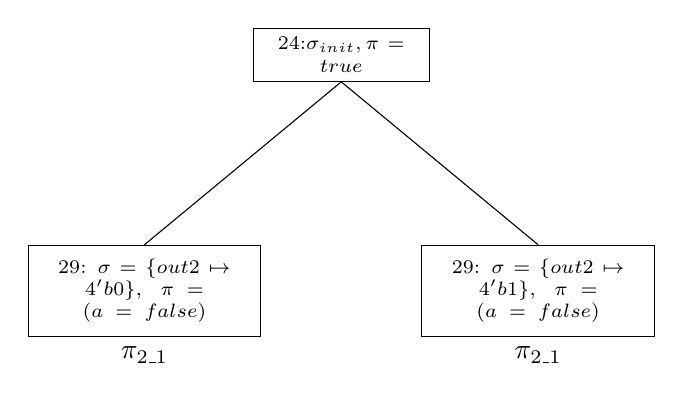
\begin{tikzpicture}[
            level 1/.style = {sibling distance=50mm, level distance=30mm}
        ]            
        %\node [draw, circle, font=\tiny] {24}
        \node [text width=20mm, align=center, draw, rectangle, font=\scriptsize]{24:$\sigma_{init}, \pi=true$}
            child {
                node [text width=26mm, align=center, draw, rectangle, font=\scriptsize, inner sep=5pt, label=below:$\pi_{2\_1}$]{29: $\sigma=\{out2 \mapsto 4'b0\},\ \  \pi=(a=false)$ }
            }
            child {
                node [text width=26mm, align=center, draw, rectangle, font=\scriptsize, inner sep=5pt,label=below:$\pi_{2\_1}$]{29:\- $\sigma=\{out2 \mapsto 4'b1\},\ \  \pi=(a=false)$ }
            };
            %child {node [draw, circle, font=\tiny, label=below:$\pi_{2\_1}$]{25}}
            %child {node [draw, circle, font=\tiny, label=below:$\pi_{2\_2}$]{27}};
            
        \end{tikzpicture}
        \label{fig:paths-b}
    }
}
\caption{All possible paths of the example module}
\label{fig:path-all}
\end{figure*}

\begin{figure}[h!]
\begin{framed}
    %\begin{lstlisting}[caption={Warm-up Verilog code}]
    \begin{lstlisting}[basicstyle=\ttfamily\tiny,backgroundcolor=]
    module comb_example(
        input  wire [3:0] a, b, c,
        output reg  [3:0] out0, out1, out2
    );
        reg [3:0] temp0;
        always @(*) begin
            if (a) begin
                temp0 = b;
            end else begin
                temp0 = 4'b0;
            end
            if (temp0 & a == 4'b1) begin
                out0 = a;
            end else begin
                out0 = 4'b1;
            end
            if (c) begin
                out1 = 4'b1;
            end else begin
                out1 = b;
            end
        end
        always @(*) begin
            if (b) begin
                out2 = 4'b1;
            end else begin
                out2 = 4'b0;
            end
        end
    endmodule
    \end{lstlisting}
\end{framed}
\caption{Motivating Verilog Code}
\label{fig:verilog-fig}
\vspace{-20pt}
\end{figure}


However, we noticed that in Figure \ref{fig:paths-a}, there still remains different paths, such as $\pi_{1\_1}$ and $\pi_{1\_5}$ , $\pi_{1\_2}$ and $\pi_{1\_6}$, $\pi_{1\_3}$ and $\pi_{1\_7}$, $\pi_{1\_4}$ and $\pi_{1\_8}$ ending with the same output state respectively. For example, when the path $\pi_{1\_1}$ is explored, $\pi_{1\_5}$ becomes redundant. 

The reasons making redundant paths in the first always block are summarized below:
\begin{itemize}
    \item The always block represents a combinational logic that consists of blocking assignments which are executed sequentially.
    \item Conditional branches $Br_7$ and $Br_{12}$ can not affect the assignment of $out1$, which is only affected by $Br_{17}$. %Hence $Br_{17}$ is independent of $Br_7$ and $Br_{12}$ .
\end{itemize}

Hence, analyzing how branch decisions propagate through the combinational logic enables us to identify redundant paths. In Section 3,  we propose a dataflow-guided exploration strategy that leverages these interactions between conditional branches to steer path
exploration, thereby avoiding redundant path explorations.

\vspace{-3mm}
\section{Dataflow-based Explore Strategy}
\label{sec:strategy}
\subsection{Overview}

%The core idea of our dataflow-guided search strategy is to reduce redundant path explorations in symbolic execution by leveraging the independence between branches within combinational logic circuits. Traditional symbolic execution explores all feasible paths exhaustively, leading to significant overhead due to path explosion. While existing approaches like Sylvia mitigate this issue by exploiting parallelism in independent always blocks, they fail to address redundancy within a single block where independent branches may generate overlapping states.
The core of our exploration strategy is to identify and prune the redundant paths during the process of symbolic execution by utilizing the dataflow analysis within combinational logic circuits. During the process of symbolic execution, we maintains a decision sequence for current path, and the exploration strategy is carried out according to the result of dataflow analysis and the decision sequence.%While existing approaches like Sylvia alleviates this issue by exploiting parallelism in independent always blocks, they fail to address redundancy within a single block where independent branches may generate overlapping states.

%The workflow of our method is shown in Figure \ref{fig:Work Flow of dataflow-guided Explore Strategy}. %First, we develop a customized dataflow analysis for hardware design, to generate a control flow graph and caculate the effect of each branch. These summaries are obtained by solving a standard forward dataflow problem over a bit-vector abstract domain through which we records every statements in RTL. Then the summary is fed into the symbolic execution engine which maintains a compact representation of the decisions taken along each path. During the symbolic execution, when countering each branch point leading different paths, we check whether the path is redundant by current decision sequence and the summary of the dataflow analysis. 
In this section,  We first show the dataflow abstraction by defining the abstract domain. Based on this abstraction, we show how to compute the summary. Finally, we provide the algorithm to check whether a path can be pruned.

%To determine independence relations among branches in the hardware design, we conduct a static dependence analysis on the RTL design to learn whether two branches are independent before the path exploration. For example, $Br_{17}$ is independent of $Br_7$ and $Br_{12}$. However, for complex designs, an explicit algorithm is required. We provide algorithm \ref{alg:independent_branch_set_calculation} in Section 3.2 to discover the independence relations between branches.





%\subsection{Dependency Graph and Dataflow Abstraction}
\subsection{Dataflow Abstraction}
\label{subsec:dataflow-abstraction}
% 抽象域 + In/Out/Gen 方程
To reason about how control decisions may affect the rest of the design,
we first construct a directed graph over the RTL design and define a
lightweight dataflow abstraction on top of it.

Let $V$ denote the set of statements in the RTL design, $Br \subseteq V$ denotes the subset of branch conditions. We consider a directed graph $G = (V, E)$,
where an edge $(u, v) \in E$ indicates that executing $u$ may have an
effect on the behavior at $v$ with respect to the observation of
interest (e.g., the values of target registers at the end of a cycle).
We build the concrete graph $G$ using existing analysis of data and control propagation in RTL. However, our pruning strategy itself only relies on $G$ as an abstract interface, to analyze the possible effects among statements in RTL.

For each node $v \in V$,  we associate a set $Out(v) \subseteq Br$ of branch statements whose decisions can reach $v$
through the directed graph and may have an impact on its behavior. Intuitively, $Out(v)$ is the \emph{decision-impact set} at node $v$.
The global abstract state is a mapping$\Delta : V \to 2^{Br}$.

Hence, $\Delta(v)$ for the current approximation of $Out(v)$ at node $v$. It is convenient to view $\Delta$ as a $|V| \times |Br|$ bit matrix, where the entry at $(v, b)$ is $1$ iff $b \in \Delta(v)$.
We treat all such mappings as elements of our abstract domain
$D = (2^{Br})^{V}$, i.e., the set of all functions that assign to each
node $v \in V$ a subset of branch nodes.
equipped with the pointwise subset order:
\[
  \Delta_1 \sqsubseteq \Delta_2
  \;\Longleftrightarrow\;
  \forall v \in V.\;\Delta_1(v) \subseteq \Delta_2(v).
\]
The join operator is pointwise union, and the bottom element $\bot$
maps every node to the empty set. This abstraction can be utilized to record \emph{which} branch decisions may reach
for each node, without tracking their concrete values or the detailed symbolic state.
\subsection{Fixed-Point Computation of Decision-Influence Summaries}
\label{subsec:fixpoint-summaries}

Given the directed graph $G = (V,E)$ and the set of branch nodes
$Br \subseteq V$, we now describe how to compute a summary for each branch. This summary indicates the effect of a branch. The computation is a forward may-analysis on the abstract domain $D$ defined in Section~\ref{subsec:dataflow-abstraction}.

For each node $v \in V$, we maintain an ``in'' and ``out'' fact,
$In(v)$ and $Out(v)$, both subsets of $Br$. Intuitively, $In(v)$
collects all decisions(taken or not taken) of branches whose effects may reach $v$ through
predecessors in the directed graph, while $Out(v)$ augments this set
with the local decision at $v$ itself when $v$ is a branch node.

The dataflow equations are $In(v) = \bigcup_{(u, v) \in E} Out(u)$ and $Out(v) = In(v) \cup Gen(v)$, where $Gen(v)$ denotes the set of facts generated
locally at node $v$: concretely, $Gen(v) = \{v\}$ when $v \in Br$ and $Gen(v) = \emptyset$ otherwise. Equivalently, over the whole RTL we
seek a mapping $Out : V \to 2^{Br}$ such that, for every $v \in V$, the equation $Out(v) = \left(\bigcup_{(u, v) \in E} Out(u)\right) \cup Gen(v)$ holds simultaneously. Essentially, solving this system of equations is a problem to fixpoint of the transfer functions on the abstract domain $D$. We adopt the standard work-list style iteration: starting from the least informative abstract state (where all $In(v)$ and $Out(v)$ are empty), we repeatedly apply the equations along the edges of $G$ and accumulate branch information until no $Out(v)$ changes. 

Algorithm\ref{alg:dataflow_influence} summarizes the fixed-point
computation. We initialize all facts to the empty set and repeatedly
propagate information along the edges of $G$ until no $Out(v)$ changes.
Because the abstract domain $D$ is finite and the transfer functions are
monotone with respect to $\sqsubseteq$, the iteration converges to the
least fixpoint. At this fixpoint, the set
$Out(v)$ is a conservative approximation of all branch
nodes whose decisions may influence node $v$.

While the union operations ensure a conservative over-approximation (maintaining soundness), they do introduce a loss of precision. Specifically, the influence sets might overestimate the actual dependencies, leading the engine to assume a branch is influenced when it concretely is not. Consequently, this precision loss only means we might miss some opportunities to prune redundant paths, but it guarantees that we will never incorrectly prune a path that contains unique, unexplored behaviors.



\begin{algorithm}[H]
    \small
    \caption{ComputeBranchInfluence}
    \label{alg:dataflow_influence}
    \begin{algorithmic}[1]
    \Require Directed graph $G = (V, E)$, branch set $Br \subseteq V$
    \Ensure $Out(v)$ for all $v \in V$, and $InflNodes(Br)$ for all $Br \in Br$
    
    \State \textbf{for all} $v \in V$: $In[v] \gets \emptyset$, $Out[v] \gets \emptyset$
    
    \Repeat
        \For{$v$ in $V$}
            \State $In[v] \gets \bigcup_{(u,v)\in E} Out[u]$
            \State $Gen \gets \{v\}$ \textbf{if} $v \in Br$ \textbf{else} $\emptyset$
            \State $NewOut \gets In[v] \cup Gen$
            \If{$NewOut \neq Out[v]$}
                \State $Out[v] \gets NewOut$
            \EndIf
        \EndFor
    \Until{no $Out[\cdot]$ changed in the last iteration}
    
    %\State \textbf{for all} $v \in V$: $DepBr[v] \gets Out[v]$
    \State \textbf{for all} $Br \in Br$: $InflNodes[Br] \gets \emptyset$
    
    \For{$v$ in $V$}
        %\For{$Br$ in $DepBr[v]$}
        \For{$Br$ in $Out[v]$}
            \State $InflNodes[Br] \gets InflNodes[Br] \cup \{v\}$
        \EndFor
    \EndFor
    
    %\State \Return $(DepBr, InflNodes)$
    \State \Return $(Out, InflNodes)$
    \end{algorithmic}
\end{algorithm}
\vspace{-3mm}
Based on $Out(v)$, we then derive, for each branch $b \in Br$, a
decision--influence summary $InflNodes(b)$ that collects all nodes potentially affected by $b$. These summaries will be used by the symbolic execution engine to compare decision histories and to identify observationally redundant paths.

According Algorithm\ref{alg:dataflow_influence}, we can caculate a summary for each branch statement in the motivating example. For example, $InflNodes(Br_7) = \{Br_7, 8, 10, Br_{12}, 13, 15\}$, $InflNodes(Br_12) = \{ Br_{12}, 13, 15\}$, $InflNodes(Br_{17}) = \{ Br_{17}, 18, 20\}$ and $InflNodes(Br_{24}) = \{ Br_{24}, 25, 27\}$.  In particular, they show that the influence regions of $Br_{17}$ and $Br_{24}$ are disjoint from those of $Br_{7}$ and $Br_{12}$, whereas $Br_{7}$ and $Br_{12}$ share a common influence region around the computation of \texttt{out0}.
\vspace{-3mm}
\subsection{Symbolic Execution with Dataflow-Guided Pruning}
\label{subsec:symex-pruning}
In this subsection we describe how the summaries $InflNodes(\cdot)$ are integrated into the symbolic execution engine. The engine follows a standard path-based scheme: for each path $\pi$, it maintains a path condition $pc_\pi$ and a symbolic state $\sigma_\pi$, and forks execution whenever it encounters a branch statement. In our framework, each symbolic state is additionally annotated with the set of branch nodes whose outcomes have already been fixed along the path. We use $ExecutedBranches(\pi) \subseteq Br$ to represent the set of branch statements, which can be extracted from $pc_\pi$; intuitively, $ExecutedBranches(\pi)$ summarizes the history of control decisions taken so far on path $\pi$.

When the executor reaches a branch node $b \in Br$, it invokes a
dataflow-guided pruning procedure before actually forking the state.
The procedure, shown in Algorithm~\ref{alg:prune_strategy_df}, checks
whether exploring $b$ under the current history can lead to any new
abstractly distinguishable behavior. Concretely, it (i) tests whether
the influence region of $b$ overlaps with the influence region of any
previously executed branch along the current path, by inspecting the
precomputed sets $InflNodes(\cdot)$; if
$InflNodes(b) \cap InflNodes(b') \neq \emptyset$ for some
$b' \in ExecutedBranches(\pi)$, then the effects of $b$ may interact
with those of $b'$, and the pruning rule is not triggered. Otherwise
(the influence region of $b$ is disjoint, at the abstract level, from
all previously affected nodes), it (ii) consults a bookkeeping
predicate $\mathit{FullyExplored}$ to decide whether all local
sub-paths stemming from $b$ have already been explored under histories
that are compatible with the current one; if so, exploring $b$ again
cannot reveal new abstract behaviors and the current path can be safely
pruned, otherwise exploration continues.

Unlike software symbolic execution, where identical outputs might obscure divergent side effects (e.g., memory corruption), RTL combinational logic is fully deterministic within a clock cycle. If two paths produce identical updates to all influenced variables, their resulting hardware states at the clock boundary are strictly identical, ensuring that our pruning strategy is sound and introduces no false negatives.




\noindent
The structure \textit{BranchCoverage} and the predicate \textit{FullyExplored} are implemented on top of the existing path
management logic; they record, for each branch, which combinations of local outcomes and compatible histories have already been visited.
\vspace{-4pt}
\begin{algorithm}[]
    \small
    \caption{ControlFlowPrune}
    \label{alg:prune_strategy_df}
    \begin{algorithmic}[1]
    \Require $InflNodes$, current branch $Br$, current state $s$, bookkeeping structure $BranchCoverage$
    \Ensure True or false 
    \Comment{The path can be pruned when the output is True}
    
    \State $ExecutedBranches \gets GetBranch(s.pcon)$
    \Statex \hspace{\algorithmicindent}\Comment{GetBranch analyzes $s.pcon$ to obtain the branches along the current path}

    
    \For{$Br'$ in $ExecutedBranches$}
        \If{$InflNodes[Br] \cap InflNodes[Br'] \neq \emptyset$}
            %\Comment{Effects of $Br$ may interact with an existing decision}
            \State \Return false
        \EndIf
    \EndFor
    
    \If{FullyExplored(Br, ExecutedBranches, BranchCoverage)}
        %\Comment{All relevant local sub-paths of $Br$ under compatible histories have been explored}
        \State \Return true
    \Else
        \State \Return false
    \EndIf
    
    \State \Return false
    \end{algorithmic}
\end{algorithm}

\vspace{-3mm}

\section{Evaluation}
\label{sec:evaluation}
We implemented our approach on the top of a symbolic execution engine, Sylvia \cite{Ryan2023Sylvia}, which is a symbolic execution engine for hardware verification and built in Python3.8. Sylvia analyzes the RTL of the hardware designs by pySlang. We integrated our dataflow-based exploration strategy into Sylvia, and evaluated the performance of our approach on 3 RTL design: two RISC-V cores(the PICORV32, and a old version of DarkRISCV) and a SoC design from Hack@DAC'18. We compared the performance of our approach with Sylvia by measuring the time and space consumption, as well as the number of paths explored.Since the huge complexity of HACK@DAC'18, which is an SoC design, it is impossible to explore all the paths that it can reach, we evaluate our method by finding assertion violations. Once find the violation, the process of exploration will stop. Then we compare the time and space consumption, as well as the number of paths explored of these two methods. The assertions we used can be found in an open-sourced benchmark\cite{rogers2025hardware}.
\subsection{Experimental Setup}
%We mainly evaluate the performance of our approach on 3 RTL design: two RISC-V cores(the PICORV32, and a old version of DarkRISCV) and a SoC design from Hack@Dac'18. 
%The expriments are conducted on a compputer with AMD Ryzen 9 9950x3d CPU, 96GB RAM and the operating system is Ubuntu 24.04. The symbolic execution engine is implemented in Python3.12.3, and the SMT solver is Z3. We use the pySlang, to analyze the System Verilog code.
Experiments were performed on a machine with an AMD Ryzen 9 9950X3D CPU, 96GB RAM, and Ubuntu 24.04. The symbolic execution engine, implemented in Python 3.12, used the Z3 SMT solver and pySlang to analyze SystemVerilog.

Table \ref{tab1_1} presents the structure of three RTL designs mentioned above. Columns of Design,  LoC, Branch Points, and Always Blocks represents the line of code, total counts of the branch and number of always blocks, respectively.
\begin{table}[ht]
    \centering
    \begin{tabular}{l|c|c|c}
    \hline
    Design & LoC & Branch Points & Always Blocks \\
    \hline
    PICORV32 & 2193 & 230 & 29 \\
    \hline
    DarkRISCV & 531 & 51 & 2 \\
    \hline
    Hack@DAC2018 & 96444 & 4452 & 883 \\
    \hline
    \end{tabular}
    \vspace{5pt}
    \caption{Structures of benchmark}
    \label{tab1_1}
\end{table}
\vspace{-20pt}
%并列柱状图

\subsection{Effects of Optimizations}
% The reason we utilize DeepSeek to generate the testcases is to make a high diversity of combinations of dependence relations in the design. After that, we evaluate PICORV32 and DarkRISCV, two open-source RISC-V cores, to see what can our method achieve in a real core. These experiments study the effectiveness of our exploration strategy against Sylvia, in terms of total number of explored paths, times of SMT query, consumptions of time and memory during exploration.


%Figure \ref{fig:sub2} demonstrates how our methods reduce the total number of SMT queries. Reducing the number of explored paths also reduces the total SMT queries. The effect of reduction on SMT queries is not positive correlation with the reduction on total amount of explored paths. %For example, StateController decrease 40\% of total path and 26.5\% of total amount of SMT queries, but testcase1 decreases 50\% of total amount of SMT queries with reduction of 50\% on pruned paths.

We evaluate our method against Sylvia on the two open-sourced RISC-V cores, and a SoC design, to study the effectiveness of our strategy of exploration. Path of exploration, times of SMT queries, total run time and total memory usage are the criteria that we focus on. For both designs, we first count the LoC(lines of code) and the amounts of branch points and always blocks in Table \ref{tab1_1}. PICORV32 is a more complex design since the LoC, the number of branch point and always blocks of PICORV32 are multiple times of DarkRISCV.



%    Sylvia & 5802 & 246738 & 64sec & 1286MB \\
%    \hline
%    dataflow-guided Prune & 4906 & 180646 & 54sec & 1508MB \\

\begin{figure*}[t]
    \centering
    % 子图 1
    \subfigure[Paths of Exploration]{
        \includegraphics[width=0.23\textwidth]{paths.jpg}
        \label{fig:sub1}
    }
    \hfill
    % 子图 2
    \subfigure[SMT Query Times]{
        \includegraphics[width=0.23\textwidth]{smtQuery.jpg}
        \label{fig:sub2}
    }
    \hfill
    % 子图 3
    \subfigure[Run Time]{
        \includegraphics[width=0.23\textwidth]{runTime.jpg}
        \label{fig:sub3}
    }
    \hfill
    % 子图 4
    \subfigure[Memory Usage]{
        \includegraphics[width=0.23\textwidth]{memory.jpg}
        \label{fig:sub4}
    }

    \caption{Comparison between Sylvia and dataflow-guided pruning on PICORV32, DarkRISCV and HACK@DAC'18.}
    \label{fig:four-subfigures}
\end{figure*}



The experimental results on the PICORV32 benchmark demonstrate that the dataflow-guided pruning approach reduces the number of exploration paths by 9.9\% (from 4992 to 4498), decreases query times by 38.1\% (from 194,524 to 120,428), and shortens the run time by 25.3\% (from 145.17 seconds to 108.39 seconds) compared to the Sylvia method, albeit at the cost of a 21.0\% increase in memory consumption (from 425,164 KB to 514,340 KB). On the Darkriscv, dataflow-guided pruning achieves more substantial reductions in exploration paths (33.9\%, from 73,600 to 48,648) and run time (36.7\%, from 512.36 seconds to 324.32 seconds), while the reduction in query times is 25.1\% (from 601,580 to 450,428) and the memory overhead is limited to 9.8\% (from 2,886,608 KB to 3,169,634 KB). These results indicate that dataflow-guided pruning is particularly effective for larger designs, yielding greater improvements in path reduction and run time efficiency with relatively lower memory overhead growth.
At the first glance, it is surprising to see that DarkRISCV consumes much more resources than PICORV32. The paths of exploration on DarkRISCV is about 14 times than the amount of paths on PICORV32. After analyzing the structures of the designs, we find that it is the amount of always blocks causes this circumstance. More always blocks make Sylvia to reduce more paths to explore. This difference somehow inspire us there is a huge space to reduce the redundant paths if we leverage the characteristics of hardware. 

The experimental results on the Hack@DAC2018 benchmark show that the dataflow-guided pruning approach reduces the number of exploration
paths by 15.4\% (from 5,802 to 4,906), decreases query times by 26.8\% (from 246,738 to 180,646), and shortens the run time by 15.6\%
(from 64 seconds to 54 seconds) compared to the Sylvia method, while incurring a 17.3\% increase in memory usage (from 1,286 MB to 1,508 MB). 
The observed 10–20\% memory overhead is an expected trade-off for maintaining decision-impact sets and path histories, yielding substantial runtime and query reductions. To scale to massive industrial SoCs, future implementations can mitigate potential memory bottlenecks by periodically flushing these influence summaries once execution paths within a localized combinational block fully converge.
%Based on the results of three RTL design, the observed increase in memory usage is expected and stems directly from the additional data structures required by our dataflow-guided pruning, such as per-node decision-impact sets and the bookkeeping needed to track previously explored decision histories. In other words, our technique deliberately trades a moderate amount of extra memory for substantial reductions in explored paths, SMT queries, and runtime. Across all benchmarks, this time–memory trade-off remains well-behaved: the memory overhead stays within 10--20\%, while the savings in search effort and execution time are significantly larger. For industrial-scale designs where this memory overhead might potentially become a bottleneck, the trade-off can be dynamically managed. Future implementations could easily mitigate this by periodically flushing the influence summaries and branch histories once execution paths within a localized combinational block fully converge, thereby ensuring scalability for massive SoCs.
\vspace{-5pt}

\section{Related Work}
\label{sec:related_work}
Symbolic execution is a popular technique in both software and hardware verification. Since it can reach a deep depth of verification and achieve a high coverage, symbolic execution are widely used for the security verification of hardware designs.

\paragraph{Symbolic Execution and Concrete Test}
As a mix of symbolic execution and concrete testing, concolic testing uses concrete values to replace some symbolic variables to avoid the analysis of unnecessary paths. QUEBS\cite{concolic_1} prevents path explosion by limiting the number of times a branch can be selected. Lyu and Mishra \cite{concolic_3} proposed an approach maps directed test generation problem to target search problem to search by learning and clustering techniques to reduce the overlapping searches.% Meng and Kundu \cite{concolic_3} generated security test cases for identifying critical exploits manifested in a System on Chip. 

%\paragraph{Symbolic Execution and Fuzzing}
%Symbolic execution hybrids with fuzzing technique as well to quickly enumerate inputs without heavy constraint solving. Dai, and Yavuz \cite{fuzzing_1} employed fuzzing and static analysis to generate models of suspicious hardware elements that are used as oracles to guide symbolic execution.  Jingxuan He and Gishor Sivanrupan et al. \cite{fuzzing_2}used tests generated by LEARCH as initial fuzzing seeds enables the popular fuzzer AFL\cite{afl} to find more paths and security violation. Specifically, LEARCH \cite{fuzzing_2} is a learning-based strategy they proposed to tackle path explosion problems by selecting promising states.

Many of works mentioned above first translate the hardware design into a software model represented as C/C++ code, , then use the symbolic execution tool, KLEE\cite{klee} targeting on software verification. The translation into software models is typically accomplished via standard commercial or open-source EDA tools.
%The translation from hardware into software models can be accomplished by EDA tools for commercial, e.g. Cadence\cite{Cadence}, Synopses\cite{Synopsys}, or open-source tools, e.g. Verilator \cite{Verilator}, Icarus Verilog \cite{iVerilog}.

\paragraph{Symbolic Execution on RTL designs}
Some works directly do symbolic execution on Verilog. RTL-ConTest \cite{concolic_3} generated security test cases for identifying critical exploits manifested in a System on Chip operates directly on the SoC RTL. They use Python to analyze the original Verilog to generate CFG to assist path selection. Sylvia\cite{Ryan2023Sylvia} utilizes pyVerilog to generate the AST of the Verilog to identify the independent always blocks. It reduces redundant paths to explore by separately explore the independent blocks. SEIF \cite{seif} take Sylvia as a framework, implements a methodology and search heuristics for information flow verification.
\vspace{-5pt}
\section{Conclusion}
\label{sec:conclusion}
%This paper presents a dataflow-guided symbolic execution for hardware verification. We first utilize dataflow analysis to discover the relations among the statements in the combinational logics in the RTL, and then we propose a pruning strategy to prune the redundant paths leading to the same states. We implement our approach on the top of a symbolic execution engine, Sylvia, and evaluate its performance on 3 RTL designs. Especially, the experimental results show that our approach can significantly reduce even 34\% of paths in DarkRISCV explored by Sylvia.
This paper introduces a dataflow-guided symbolic execution approach for hardware verification. It leverages dataflow analysis to identify relationships among statements in RTL combinational logic and employs a pruning strategy to eliminate redundant paths that lead to identical states. Implemented on top of the Sylvia symbolic execution engine, the approach is evaluated on three RTL designs. Experimental results demonstrate that it reduces the number of explored paths in DarkRISCV by 34\%.
\vspace{-5pt}
\section{ACKNOWLEDGMENT}
\label{sec:ack}
This work was supported by the National Natural Science Foundation of China (No. 62372438) and the Beijing Municipal Natural Science Foundation (No. 4252024).



\bibliographystyle{IEEEtran}
\bibliography{ref}



\end{document}
